\chapter{Theoretical background} \label{chap_theoreticalbackground} 

The goal of this thesis is to investigate whether \gls{ca} approach convergeges and aligns
with the goals of \gls{ns}. In the cource of this research there are several 

Therefore, it is essential to have a comprehensive
understanding of software stability and the key concepts, principles, and architectures
that impact software stability.

This chapter begins by describing the concepts of software stability, evolvability, and
modularity, highlighting their significance in achieving software stability in \gls{ns}.
This is followed by a brief overview of the design theorems and proposed architecture of
\gls{ns}.

The subsequent sections of the thesis explore the fundamental principles that underlie
\gls{ca}, as well as its proposed architectural designs. Finally, the thesis
concludes by discussing which aspects of \gls{ca} align with the principles of
\gls{ns} and contribute to achieving software stability in this approach.

\section{Generic Concepts} \label{section_key_concepts}

The following sections will explore the fundamental concepts of modularity, cohesion, and
coupling. These concepts are incorporated by both \gls{ca} and \gls{ns} and are 
essential to study evolvability of software artifacts.

\subsection{Modularity} \label{subsec_modularity}

The original material of \textcite[82]{robert_c_martin_clean_2018} describes a module as a
piece of code encapsulated in a source file with a cohesive set of functions and data
structures. According to \textcite[22]{mannaert_normalized_2016}, modularity is a
hierarchical or recursive concept that should exhibit high cohesion. While both design
approaches agree on the cohesiveness of a module's internal parts, there seems to be a
slight difference in granularity in their definitions.
\chapter{Component Cohesion Principles} \label{appendix_cohesion_principles}

\begin{table}[H]
    \small
    \begin{tabular}{ P{0.25\linewidth} | p{0.69\linewidth}} 
        \hline
        \textbf{Name} & \textbf{Description} \\ \hline
        \acrlong{rep} & \acrshort{rep} is a concept related to software development that
        refers to the balance between reusing existing software components and releasing
        new ones to ensure the efficient use of resources and time
        \parencite[104]{robert_c_martin_clean_2018}.\\ \midrule 
        
        \acrlong{ccp} & In the context of Clean Architecture, the \acrshort{ccp} states
        that classes or components that change together should be packaged together. In
        other words, if a group of classes is likely to be affected by the same kind of
        change, they should be grouped into the same package or module. This approach
        enhances the maintainability and modularity of the software
        \parencite[105]{robert_c_martin_clean_2018}.\\ \midrule 
        
        \acrlong{crp} & \acrshort{crp} states that classes or components that are reused
        together should be packaged together. It means that if a group of classes tends to
        be used together or has a high level of cohesion, they should be grouped into the
        same package or module. This approach aims to make it easier for developers to
        reuse components and understand their relationships
        \parencite[107]{robert_c_martin_clean_2018}.\\

        \bottomrule
    \end{tabular}
    \caption{The component Cohesion Principles}
    \label{appendix_tab_cohesion_principles}
\end{table}

Cohesion facilitates the reduction of complexity and interdependence among the components
of a system, thereby contributing to a more efficient, maintainable, and reliable system.
By organizing components around a shared purpose or function or by standardizing their
interfaces, data structures, and protocols, cohesion can offer the following benefits:

\begin{itemize}
    \item \textbf{Reduce redundancy and duplication of effort}: \\
    Cohesion ensures that components are arranged around a common purpose or function,
    reducing duplicates or redundant code. This simplifies system comprehension,
    maintenance, and modification.
    \item \textbf{Promoting code reuse:}\\
    Cohesion facilitates code reuse by making it easier to extract and reuse components
    designed for specific functions. This saves time and effort during development and
    enhances overall system quality.
    \item \textbf{Enhance maintainability:}\\
    Cohesion decreases the complexity and interdependence of system components, making it
    easier to identify and rectify bugs or errors in the code. This improves system
    maintainability and reduces the risk of introducing new errors during maintenance.
    \item \textbf{Increase scalability:}\\
    Cohesion improves a system's scalability by enabling it to be extended or modified
    effortlessly to accommodate changing requirements or conditions. By designing
    well-organized and well-defined components, developers can easily add or modify
    functionality as needed without disrupting the rest of the system.  
\end{itemize}
\subsection{Low Coupling} \label{subsec_on_coupling}

Coupling is an essential concept in software engineering related to the degree of
interdependence among software modules and components. High coupling between modules
indicates the strength of their relationship, whereby a high level of coupling implies a
significant degree of interdependence. Conversely, low coupling signifies a weaker
relationship between modules, where modifications in one module are less likely to impact
others. Although not always possible, the level of coupling between the various modules of
the system should be kept to a bare minimum. Both \textcite[23]{mannaert_normalized_2016}
and \textcite[130]{robert_c_martin_clean_2018} agree with the idea that modules should be
coupled as loosely as possible
\section{Normalized Systems Theory} \label{sec_ns_theory}

The Theory of \gls{ns} revolves around modular structures in information systems and their
behavior when modified over time. \gls{ns} uses scientific insights from System Theory and
Statistical Entropy from Thermodynamics. \gls{ns} has a background in software
engineering. However, the underlying Theory of \gls{ns} can be applied to various other
domains, such as Enterprise Engineering \parencite{huysmans_towards_2013}, Business
Process Modeling \parencite{van_nuel_towards_2011}, and the application in TCP-IP based
firewall rule base \parencite{haerens_evolvability_2021}. This emphasizes the impact that
\gls{ns} Theory has. In the following sections, we will highlight the concepts of
\gls{ns} Theory that has impacted this study.

\subsection{Stability} \label{subsec_on_stability}

\gls{ns} Theory considers stability a crucial property.
\textcite[269-270]{mannaert_normalized_2016} describe that stable software is not
excessively sensitive to small changes. The number of changes required for new versions of
the system is not dependent on the size of that system. Conversely, instabilities occur
when the total number of changes relies on the size of the system. The bigger the size of
the system, the more changes are required to implement the requirement. Mannaert et al.
\textcite[271]{mannaert_normalized_2016} refer to these instabilities' \gls{ce}
\subsection{Anticipated Changes} \label{subsec_anticipated_changes}

Conversely, instabilities occur when the total number of changes relies
on the size of the system. The bigger the size of the system, the more changes are
required to implement the requirement.\textcite[271]{mannaert_normalized_2016} refer to
these instabilities as Combinatorial Effects.
\subsection{Expansion} \label{subsec_expansion}

According to \textcite[403]{mannaert_normalized_2016}, creating and maintaining a stable
and evolvable system is a particularly challenging, repetitive, and meticulous engineering
job. Developers must have a sound knowledge of NS while implementing new requirements in
an always consistent manner. \textcite[403]{mannaert_normalized_2016} propose automating
software structure instantiation by using code generation for recurring tasks. This
process is referred to as expansion.


\subsection{The Theoretical Framework} \label{subsec_ns_desing_theorems}

\gls{ns} consists of a theoretical framework describing a set of design principles. These
principles are the basis for achieving the concepts of stability, evolvability, and
modularity. \gls{ns} provides a rigorous and mathematical foundation for these theorems
and they offer guidelines for designing and developing software systems. In the following
sections, we will focus on the principles of \gls{ns} very briefly as they have been
extensively described in various scientific papers.

We know from Chapter \ref{sec_artifact_requirements} that the design artifacts, as a part
of this research, are implemented based on the \gls{ca} principles. Therefore, contrary to
Chapter \ref{sec_ca_theory}, there will be no references to the manifestations of the NS
design theorems in the design.

\subsubsection{Separation of Concerns} \label{subsubsec_soc}

\gls{soc} as a principle has first been mentioned by
\citeauthor{dijkstra_selected_1982}\footnote{\url{https://en.wikipedia.org/wiki/Separation_of_concerns}}
as the crucial principle to design modular software architecture
\parencite[]{dijkstra_selected_1982}. \gls{soc} promotes the idea that a program should be
divided into distinct sections, each addressing a particular concern or aspect of a design
problem. This allows for a more organized and maintainable source code. When implemented
correctly, a change to one concern does not affect the others. \gls{soc} should be applied
at the level of individual modules, rather than the level of an entire program.

\gls{soc} has been adopted as one of the design theorems of \gls{ns}, although it has a
stricter definition of this principle\parencite{mannaert_normalized_2016}.

\mycolorbox{A processing function can only contain a single task to achieve stability.}{Theorem I}
\subsubsection{Data version Transparency}

\gls{dvt} is the act of encapsulation of data entities for specific tasks at hand. This
results in the fact that data structures can have multiple versions often mentioned as
Data Transfer Objects in modern software engineering projects. In other words, it should
be possible to update the data entity without affecting the processing functions. This
leads to the following description of the theorem \parencite[280]{mannaert_normalized_2016}.

\mycolorbox{A data structure that is passed through the interface of a processing function
needs to exhibit version transparency to achieve stability.}{Theorem II}

\gls{dvt} is widely used in various technological applications. practically every web
service currently known supports some type of versioning. In restful APIs, for example, it
is common practice to support versioning over the URI. It is considered a best practice to
encapsulate breaking changes in a new version of the endpoint/service so that the
consumers are not (directly) affected by the change. In modern Object Oriented languages,
gls{dtv} is also supported by the ability to determine the scope of visibility of the
modifiers of the various programming constructs like fields, properties, interfaces, and
classes, also known as information hiding
\parencites{parnas_criteria_1972}[278]{mannaert_normalized_2016}.
\subsubsection{Action version Transparency}
\gls{avt} is the property of a system to modify existing processing functions without
affecting the existing ones. It should be possible to upgrade a function without affecting
the callers of those functions. This description leads to the following theorem
\parencite[282]{mannaert_normalized_2016}.

\mycolorbox{A processing function that is called by another processing function, needs to exhibit version transparency to achieve stability.}{Theorem III}

Most of the modern technology environments support some form of \gls{avt}. Polymorphism is
a widely used technique to support this theorem. Specifically, parametric
polymorphism \footnote{\url{https://en.wikipedia.org/wiki/Parametric_polymorphism}} allows
for a processing function to have multiple input parameters. There are also quite some
design patterns supporting this theorem. Some random examples are the state pattern
\footnote{\url{https://en.wikipedia.org/wiki/State_pattern}}, facade pattern
\footnote{\url{https://en.wikipedia.org/wiki/Facade_pattern}} and observer pattern
\footnote{\url{https://en.wikipedia.org/wiki/Observer_pattern}}.
\subsubsection{Separation of State}

\gls{sos} is a theorem that is based on the idea that processing functions should not
contain any state information but instead should rely on external data structures to store
state information. By separating state information from processing functions, Normalized
Systems can achieve a higher level of flexibility and adaptability. External data
structures can be updated or replaced without affecting the processing functions
themselves, which significantly reduces the change of unwanted ripple effects. This theorem is
described as followed: \parencite[258]{mannaert_normalized_2016}.

\mycolorbox{Calling a processing function within another processing function, needs to exhibit state keeping to achieve stability.}{Theorem IV}
\subsection{The Design Elements} \label{subsec_design_elements} \todo{add cites to CA book}

\textcite{robert_c_martin_clean_2018} proposes the following elements to achieve
the goal of \enquote{Clean Architecture}.

\begin{table}[H]
    \begin{tabular}{ p{0.17\linewidth} p{0.74\linewidth}}
        \hline
        \textbf{Element} & \textbf{Description} \\ 
        \hline
        Entity & Entities are the core business objects, representing the domain's
        fundamental data.\\ \midrule

        Interactor & Interactors encapsulate business logic and represent specific actions
        that the system can perform. \\ \midrule

        RequestModel & RequestModels are used to represent the input data required by a specific
        interactor.\\ \midrule

        ViewModel & ViewModels are responsible for managing the data and behaviour of the
        user interface. \\ \midrule

        Controller & Controllers are responsible for handling requests from the user
        interface and routing them to the appropriate Interactor.\\ \midrule

        Presenter & Presenters are responsible for formatting and the data for the user
        interface.\\ \midrule

        Gateway & A Gateway provides an abstraction layer between the application and its
        external dependencies, such as databases, web services, or other external
        systems.\\ \midrule

        Boundary & Boundaries are used to separate the the different layers of the component.\\

        \bottomrule
    \end{tabular}
    \caption{The Elements proposed by Clean Architecture}
    \label{ca_element}
\end{table}
\section{Clean architecture: A design approach}\label{sec_ca_theory}

\gls{ca} is a software design approach that emphasizes the organization of code
into independent, modular layers with distinct responsibilities. This approach aims to
create more flexible, maintainable, and testable software systems by enforcing the
separation of concerns and minimizing dependencies between components. The goal of clean
architecture is to provide a solid foundation for software development, allowing
developers to build applications that can adapt to changing requirements, scale
effectively, and remain resilient against the introduction of bugs
\parencite{robert_c_martin_clean_2018}.

\section{An Analysis of Priniples} \label{sec_converging_principles}

In this section, we will apply a systematic cross-referencing approach to assess the level
of alignment between each of the principles of \gls{ca} with \gls{ns}. Along with a brief
explanation, the level of alignment is denoted as follows:

\begin{table}[H]
    \begin{tabular}{ l l p{0.57\linewidth}} 
        
    Strong alignment & \fullAlignment & This indicates that the principles of \gls{ca} and \gls{ns}
    are highly aligned. Both have a similar impact on the design and implementation of the
    artifact. \\
        
    Supports alignment & \partialAlignment & The \gls{ca} principle supports in implementing the
    \gls{ns} principle through specific design choices. However, applying the \gls{ca}
    principle does not inherently ensure adherence to the corresponding \gls{ns}
    principle. \\
        
    No or weak alignment & \noAlignment & The principles are not aligned or have no significant
    similarities in terms of their purpose, goals, or architectural supports \\
    \end{tabular}
\end{table}

\subsection{Single Responsibility Principle} \label{srp}

\evaluatePrincipleTable{\gls{srp}}{table_srp_alignment}{ \addEvalRow{\gls{soc} & \fullAlignment &
    The main goal of both \gls{srp} and \gls{soc} is to promote and encourage modularity,
    low coupling, and high cohesion. While the definition has some differences, the two
    principles can be regarded as practically interchangeable. Many examples in the
    Artifacts show a strong alignment between \gls{srp} and \gls{soc}. To name one, an
    Expander should be able to can perform multiple Tasks to complete the full
    instantiation of the Model. Each of those Tasks can be implemented separately from
    each other. Figure \ref{fig_handlers} illustrated some of the Tasks that are
    implemented in the Clean Architecture Expander Artifact. The Code Listing
    \ref{list_entityexpander} is an example of one implementation of such a Task
    \citecode{koks_expandentitieshandlerinteractor_2023}.}
    
    \addEvalRow{\gls{dvt} & \partialAlignment & Although using \gls{srp} does not
    implicitly guarantees \gls{dvt}, it does support \gls{dvt} by directing certain design
    choices. For example, both \gls{ca} and \gls{ns} assign specific \gls{dto} objects to
    support specific use cases (Interactors or Tasks) or to transfer (parts of) Data
    between architectural layers. \gls{ca} specifically assigned \glspl{dto} and
    guidelines on where and when to use them. These are also applied in the Artifact of
    this study as ResponseModels, RequestModels, and ViewModels
    \parencites{koks_requestmodels_2023,koks_viewmodels_2023}. The separation of data
    structures specific to Use Cases minimizes the impact of data structure changes by
    preferring stamp coupling over data coupling. However, \gls{srp} is not a guaranteed
    measure for \gls{dvt}.}
    
    \addEvalRow{\gls{avt} & \partialAlignment & While \gls{srp} emphasizes limiting the
    responsibility of each module, it does not explicitly require handling specific
    versions of use cases. Nevertheless, adhering to gls{srp} can still indirectly
    contribute to achieving \gls{avt}. One way to achieve this is by separating versions
    of Actions into separate contracts, objects, or methods, enabling Action Version
    transparency to some degree. Although not yet available in the Artifact, the Code
    Listing \ref{list_versioning} shows that API versioning is a common standard practice
    and fully supported by the open API specifcation and the .net core framework
    \parencites{github_aspnet-api-versioningprogramcs_2023, oas_versioning_2023}.
    Manifestations in the Artifact can be located in the Logger (Code Listing
    \ref{list_logging}), amongst others \parencite*{koks_logger_2023}.}
    
    \addEvalRow{\gls{sos} &\noAlignment & Following \gls{srp} might lead to separate modules
    that manage their state, indirectly contributing to \gls{sos}. However, the alignment
    is very weak, and no manifestations are found in the artifacts.}

}

\begin{figure}[H]
    \centering
    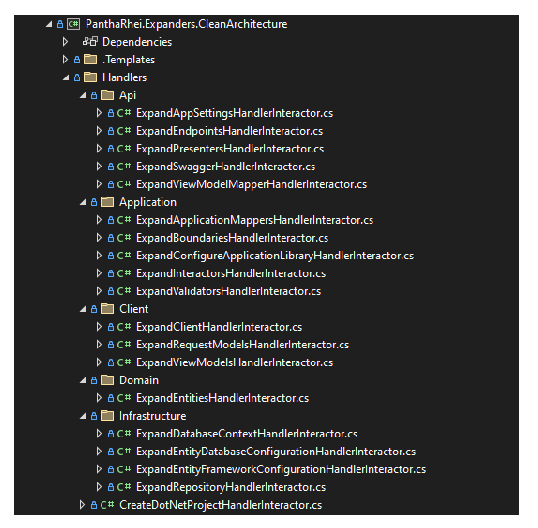
\includegraphics[width=0.6\textwidth]{figures/expander_handlers.pdf}
    \caption[handlers]{Each of the handlers handles an isolated part of the expanding process.}
    \label{fig_handlers}
\end{figure}
\subsection{Open/Closed Principle}

\evaluatePrincipleTable{\acrshort{ocp}}{table_ocp_convergence}{ 
    
\addEvalRow{\gls{soc} & \fullConvergence & The \gls{ocp} strongly converges with
    the \gls{soc} principle of \gls{ns}. \gls{ocp} states that software architectures
    should be open for extension but closed for modification. When applying \gls{ocp}
    correctly, the architecture supports new requirements built as an extension, affecting
    as few existing implementations as possible. Conversely, adhering to \gls{soc} does
    not guarantee adherence to \gls{ocp}, as \gls{soc} focuses on modularization and
    encapsulation rather than the extensibility of functionality. The same example with
    the Tasks provided in sub-section \ref{srp} is also an excellent manifestation of this
    principle.} 
    
\addEvalRow{\gls{dvt} & \noConvergence & The \gls{ocp} indirectly relates to the \gls{dvt}
principle. The convergence of both principles is weak, and no manifestations are found in
the artifacts.}
    
\addEvalRow{\gls{avt} & \fullConvergence & The \gls{ocp} strongly converges with the
    \gls{avt} principle of \gls{ns}, as both principles emphasize the importance of
    allowing changes or extensions to actions without affecting existing implementations.
    \gls{ocp} is also closely related to \gls{srp}. Besides \gls{srp}, \gls{ocp} has the
    most manifestations in the artifact, some of which are already mentioned in previous
    examples. } 
    
\addEvalRow{\gls{sos} & \noConvergence & The \gls{ocp} indirectly relates to the \gls{sos}
    principle. The convergence of both principles is weak, and no manifestations are found
    in the artifacts. } }
\subsection{Liskov Substitution Principle}

\evaluatePrincipleTable{\gls{lsp}}{table_lsp_alignment}{ 
    
\addEvalRow{\gls{soc} & \fullAlignment & \gls{lsp} states that objects of a derived class should be
able to replace objects of the base class without affecting the program negatively.
Replacing objects can only be achieved by separating them, aligning the principles
inherritly. A good example is the implementation of the
\citecode{koks_itemplateinteractor_2023} where the template engine Scriban
\parencite{github_scriban_2023} is used to generate code instantiations as a result of the
Expanding the Model \parencite{koks_scribantemplateinteractor_2023}. We could easily
replace the Scriban template engine for an other engine with only impacting the Dependency
Injection Register.}
    
\addEvalRow{\gls{dvt} & \noAlignment & The alignment between \gls{lsp} and \gls{dvt} is weak,
and no manifestations are found in the artifacts.}
    
\addEvalRow{\gls{avt} & \partialAlignment & The \gls{lsp} supports the \gls{avt} principle.
Both principles emphasize the importance of allowing the extensibility of the software
system. By adhering to \gls{lsp}, the architecture allows for class hierarchies that can
be easily extended to accommodate new (versions of) actions, which can contribute to
achieving \gls{avt}. However, adhering to \gls{lsp} alone may not guarantee full adherence
with \gls{avt}. Considder \citecode{koks_icreategateway_2023} in Code Listing
\ref{list_ICreateGatewayExamples}. The artifact contains multiple implementations of this
interface. Each implementation could be considered a different version applied to the
interface.} 
    
\addEvalRow{\gls{sos} & \noAlignment & The \gls{lsp} does not relate to the \gls{sos}
principle. The alignment of both principles is weak, and no manifestations are found in
the artifacts.} }

\subsection{Interface Segregation Principle}

\evaluatePrincipleTable{\gls{isp}}{table_isp_convergence}{ 
    
\addEvalRow{\gls{soc} & \fullConvergence & The \gls{isp} strongly converges with the
\gls{soc} principle, as both emphasize the importance of modularity and the separation of
concerns. \gls{isp} states that clients should not be forced to depend on implementation
they do not use, promoting the creation of smaller, focused interfaces. Listing
\ref{list_ispexample} shows that each \gls{crud} operation has its own interface
\parencite{koks_crudgateways_2023}.}
    
\addEvalRow{\gls{dvt} & \noConvergence & The \gls{isp} does not relate to the \gls{dvt}
principle. The convergence of both principles is weak, and no manifestations are found in
the artifacts.}
    
\addEvalRow{\gls{avt} & \npartialConvergence & The convergence between \gls{isp} and
\gls{avt} arises from the emphasis of \gls{isp} on creating targeted interfaces tailored
to specific needs. Smaller interfaces can enhance modularity and minimize unwanted side
effects when modifying Actions in the software system, positively impacting the
implementation of the \gls{avt}. For example, modifications in Actions are likely to have
a limited impact. However, adhering to \gls{isp} is not a guarantee for \gls{avt}.} 
    
\addEvalRow{\gls{sos} & \noConvergence & The \gls{isp} does not relate to the \gls{sos}
principle. The convergence of both principles is weak, and no manifestations are found in
the artifacts.} 

}
\subsubsection{The Dependency Inversion Principle} \label{subsubsec_dip} 
\textcolor{red}{
TODO: explain how dependency injection can benefit the implementation and align with
\ref{tab_convergence_dip}}

The \gls{dip} prescribes that high-level modules should not depend on low-level modules,
and that both should depend on abstractions. The principle emphasizes that the
architecture should be designed in such a way that the flow of control between the
different objects, layers and components are always from higher-level implementations
to lower-level details.

In other words, high-level implementations like business rules, should not be concerned
about low-level implementations, such as the way the data is stored or presented to the
end user. Additionally, both the high-level and low-level implementations should only
depend on abstractions or interfaces that define a contract for how they should interact
with each other \parencite[109]{robert_c_martin_clean_2018}.

This approach allows for great flexibility and a modular architecture. Modifications in
the low-level implementations will not affect the high-level implementations as long as
they still adhere to the contract defined by the abstractions and interfaces.
Similarly, changes to the high-level modules will not affect the low-level modules as long
as they still fulfill the contract. This reduces coupling and ensures the evolvability
system over time, as changes can be made to specific modules without affecting the rest of
the system.

Manifestations in the artifacts are ample. One of which is the consistent use of the
Dependency Injection pattern. In order to prevent the risks of displacing and dispersing
dependencies all over the system \parencite[214]{mannaert_normalized_2016} we are using
dependency containers. Each module is maintaining its own dependencies, which are
bootstrapped at application startup (see Listing \ref{list_dip})
\parencite{koks_generator_2023}.

\lstinputlisting[
    caption={Bootstrapping the dependencies of each component/layer of the
    generator artifact.},
    label={list_dip}]
    {Snippets/Dip.cs}

A more abstract example is the separation of required modules into separate component
libraries. This applies to both the generated and generator artifact (see Figure
\ref{fig_solutions}). The actual compliance to the \gls{dip} is how the flow of control
between the components is organized. This is accurately depicted in Figure
\ref{fig_modulair_components} \nameref{fig_modulair_components}.

\begin{figure}[H]
    \centering
    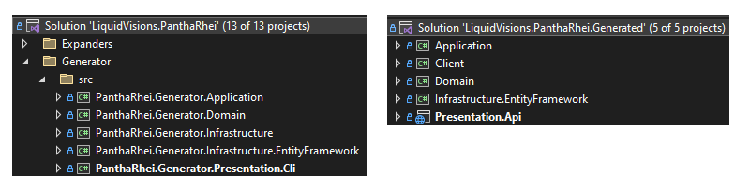
\includegraphics[width=1\textwidth]{figures/solutions.pdf}
    \caption[Separation of component libraries]{Separation of component libraries.}
    \label{fig_solutions}
\end{figure}
\subsection{The Principles Convergence Overview}

In this section, we will apply a systematic cross-referencing approach to each of the
principles of \gls{ca} with \gls{ns}. By cross-referencing these principles, we aim to
uncover the degree of convergence between \gls{ca} and \gls{ns} from a theoretical
perspective, supported by examples from the artifacts. Along with this explanation, the
level of convergence is denoted as follows:

\begin{table}[H]
\renewcommand{\arraystretch}{1.5}
\centering
\begin{tabular}{r|llll}

    \textbf{\acrlong{ca}   } \textbf{   \rotatebox[origin=l]{90}{\acrlong{ns}}} & 
    \rotatebox[origin=l]{90}{\acrlong{soc}} & \rotatebox[origin=l]{90}{\acrlong{dvt}} &
    \rotatebox[origin=l]{90}{\acrlong{avt}} & \rotatebox[origin=l]{90}{\acrlong{sos}} \\
\midrule


\acrlong{srp} & \fullConvergence & \npartialConvergence & \npartialConvergence & \noConvergence \\
\acrlong{ocp} & \fullConvergence & \noConvergence & \fullConvergence & \noConvergence \\
\acrlong{lsp} & \fullConvergence & \noConvergence & \npartialConvergence & \noConvergence \\
\acrlong{isp} & \fullConvergence & \noConvergence & \npartialConvergence & \noConvergence \\
\acrlong{dip} & \fullConvergence & \noConvergence & \npartialConvergence & \noConvergence \\
\bottomrule
\end{tabular}
\caption{An overview of the convergence of all \gls{ca} and \gls{ns} principles}
\label{tab_convergence_principles_summarized}
\end{table}



\subsection{Single Responsibility Principle} \label{srp}

\evaluatePrincipleTable{\gls{srp}}{table_srp_alignment}{ \addEvalRow{\gls{soc} & \fullAlignment &
    The main goal of both \gls{srp} and \gls{soc} is to promote and encourage modularity,
    low coupling, and high cohesion. While the definition has some differences, the two
    principles can be regarded as practically interchangeable. Many examples in the
    Artifacts show a strong alignment between \gls{srp} and \gls{soc}. To name one, an
    Expander should be able to can perform multiple Tasks to complete the full
    instantiation of the Model. Each of those Tasks can be implemented separately from
    each other. Figure \ref{fig_handlers} illustrated some of the Tasks that are
    implemented in the Clean Architecture Expander Artifact. The Code Listing
    \ref{list_entityexpander} is an example of one implementation of such a Task
    \citecode{koks_expandentitieshandlerinteractor_2023}.}
    
    \addEvalRow{\gls{dvt} & \partialAlignment & Although using \gls{srp} does not
    implicitly guarantees \gls{dvt}, it does support \gls{dvt} by directing certain design
    choices. For example, both \gls{ca} and \gls{ns} assign specific \gls{dto} objects to
    support specific use cases (Interactors or Tasks) or to transfer (parts of) Data
    between architectural layers. \gls{ca} specifically assigned \glspl{dto} and
    guidelines on where and when to use them. These are also applied in the Artifact of
    this study as ResponseModels, RequestModels, and ViewModels
    \parencites{koks_requestmodels_2023,koks_viewmodels_2023}. The separation of data
    structures specific to Use Cases minimizes the impact of data structure changes by
    preferring stamp coupling over data coupling. However, \gls{srp} is not a guaranteed
    measure for \gls{dvt}.}
    
    \addEvalRow{\gls{avt} & \partialAlignment & While \gls{srp} emphasizes limiting the
    responsibility of each module, it does not explicitly require handling specific
    versions of use cases. Nevertheless, adhering to gls{srp} can still indirectly
    contribute to achieving \gls{avt}. One way to achieve this is by separating versions
    of Actions into separate contracts, objects, or methods, enabling Action Version
    transparency to some degree. Although not yet available in the Artifact, the Code
    Listing \ref{list_versioning} shows that API versioning is a common standard practice
    and fully supported by the open API specifcation and the .net core framework
    \parencites{github_aspnet-api-versioningprogramcs_2023, oas_versioning_2023}.
    Manifestations in the Artifact can be located in the Logger (Code Listing
    \ref{list_logging}), amongst others \parencite*{koks_logger_2023}.}
    
    \addEvalRow{\gls{sos} &\noAlignment & Following \gls{srp} might lead to separate modules
    that manage their state, indirectly contributing to \gls{sos}. However, the alignment
    is very weak, and no manifestations are found in the artifacts.}

}

\begin{figure}[H]
    \centering
    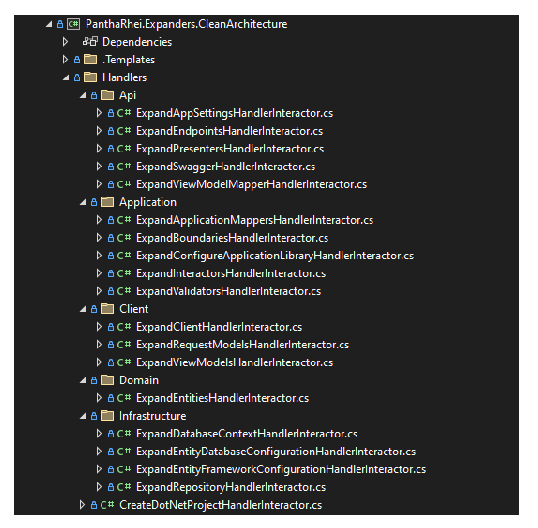
\includegraphics[width=0.6\textwidth]{figures/expander_handlers.pdf}
    \caption[handlers]{Each of the handlers handles an isolated part of the expanding process.}
    \label{fig_handlers}
\end{figure}
\subsection{Open/Closed Principle}

\evaluatePrincipleTable{\acrshort{ocp}}{table_ocp_convergence}{ 
    
\addEvalRow{\gls{soc} & \fullConvergence & The \gls{ocp} strongly converges with
    the \gls{soc} principle of \gls{ns}. \gls{ocp} states that software architectures
    should be open for extension but closed for modification. When applying \gls{ocp}
    correctly, the architecture supports new requirements built as an extension, affecting
    as few existing implementations as possible. Conversely, adhering to \gls{soc} does
    not guarantee adherence to \gls{ocp}, as \gls{soc} focuses on modularization and
    encapsulation rather than the extensibility of functionality. The same example with
    the Tasks provided in sub-section \ref{srp} is also an excellent manifestation of this
    principle.} 
    
\addEvalRow{\gls{dvt} & \noConvergence & The \gls{ocp} indirectly relates to the \gls{dvt}
principle. The convergence of both principles is weak, and no manifestations are found in
the artifacts.}
    
\addEvalRow{\gls{avt} & \fullConvergence & The \gls{ocp} strongly converges with the
    \gls{avt} principle of \gls{ns}, as both principles emphasize the importance of
    allowing changes or extensions to actions without affecting existing implementations.
    \gls{ocp} is also closely related to \gls{srp}. Besides \gls{srp}, \gls{ocp} has the
    most manifestations in the artifact, some of which are already mentioned in previous
    examples. } 
    
\addEvalRow{\gls{sos} & \noConvergence & The \gls{ocp} indirectly relates to the \gls{sos}
    principle. The convergence of both principles is weak, and no manifestations are found
    in the artifacts. } }
\subsection{Liskov Substitution Principle}

\evaluatePrincipleTable{\gls{lsp}}{table_lsp_alignment}{ 
    
\addEvalRow{\gls{soc} & \fullAlignment & \gls{lsp} states that objects of a derived class should be
able to replace objects of the base class without affecting the program negatively.
Replacing objects can only be achieved by separating them, aligning the principles
inherritly. A good example is the implementation of the
\citecode{koks_itemplateinteractor_2023} where the template engine Scriban
\parencite{github_scriban_2023} is used to generate code instantiations as a result of the
Expanding the Model \parencite{koks_scribantemplateinteractor_2023}. We could easily
replace the Scriban template engine for an other engine with only impacting the Dependency
Injection Register.}
    
\addEvalRow{\gls{dvt} & \noAlignment & The alignment between \gls{lsp} and \gls{dvt} is weak,
and no manifestations are found in the artifacts.}
    
\addEvalRow{\gls{avt} & \partialAlignment & The \gls{lsp} supports the \gls{avt} principle.
Both principles emphasize the importance of allowing the extensibility of the software
system. By adhering to \gls{lsp}, the architecture allows for class hierarchies that can
be easily extended to accommodate new (versions of) actions, which can contribute to
achieving \gls{avt}. However, adhering to \gls{lsp} alone may not guarantee full adherence
with \gls{avt}. Considder \citecode{koks_icreategateway_2023} in Code Listing
\ref{list_ICreateGatewayExamples}. The artifact contains multiple implementations of this
interface. Each implementation could be considered a different version applied to the
interface.} 
    
\addEvalRow{\gls{sos} & \noAlignment & The \gls{lsp} does not relate to the \gls{sos}
principle. The alignment of both principles is weak, and no manifestations are found in
the artifacts.} }

\subsection{Interface Segregation Principle}

\evaluatePrincipleTable{\gls{isp}}{table_isp_convergence}{ 
    
\addEvalRow{\gls{soc} & \fullConvergence & The \gls{isp} strongly converges with the
\gls{soc} principle, as both emphasize the importance of modularity and the separation of
concerns. \gls{isp} states that clients should not be forced to depend on implementation
they do not use, promoting the creation of smaller, focused interfaces. Listing
\ref{list_ispexample} shows that each \gls{crud} operation has its own interface
\parencite{koks_crudgateways_2023}.}
    
\addEvalRow{\gls{dvt} & \noConvergence & The \gls{isp} does not relate to the \gls{dvt}
principle. The convergence of both principles is weak, and no manifestations are found in
the artifacts.}
    
\addEvalRow{\gls{avt} & \npartialConvergence & The convergence between \gls{isp} and
\gls{avt} arises from the emphasis of \gls{isp} on creating targeted interfaces tailored
to specific needs. Smaller interfaces can enhance modularity and minimize unwanted side
effects when modifying Actions in the software system, positively impacting the
implementation of the \gls{avt}. For example, modifications in Actions are likely to have
a limited impact. However, adhering to \gls{isp} is not a guarantee for \gls{avt}.} 
    
\addEvalRow{\gls{sos} & \noConvergence & The \gls{isp} does not relate to the \gls{sos}
principle. The convergence of both principles is weak, and no manifestations are found in
the artifacts.} 

}
\subsubsection{The Dependency Inversion Principle} \label{subsubsec_dip} 
\textcolor{red}{
TODO: explain how dependency injection can benefit the implementation and align with
\ref{tab_convergence_dip}}

The \gls{dip} prescribes that high-level modules should not depend on low-level modules,
and that both should depend on abstractions. The principle emphasizes that the
architecture should be designed in such a way that the flow of control between the
different objects, layers and components are always from higher-level implementations
to lower-level details.

In other words, high-level implementations like business rules, should not be concerned
about low-level implementations, such as the way the data is stored or presented to the
end user. Additionally, both the high-level and low-level implementations should only
depend on abstractions or interfaces that define a contract for how they should interact
with each other \parencite[109]{robert_c_martin_clean_2018}.

This approach allows for great flexibility and a modular architecture. Modifications in
the low-level implementations will not affect the high-level implementations as long as
they still adhere to the contract defined by the abstractions and interfaces.
Similarly, changes to the high-level modules will not affect the low-level modules as long
as they still fulfill the contract. This reduces coupling and ensures the evolvability
system over time, as changes can be made to specific modules without affecting the rest of
the system.

Manifestations in the artifacts are ample. One of which is the consistent use of the
Dependency Injection pattern. In order to prevent the risks of displacing and dispersing
dependencies all over the system \parencite[214]{mannaert_normalized_2016} we are using
dependency containers. Each module is maintaining its own dependencies, which are
bootstrapped at application startup (see Listing \ref{list_dip})
\parencite{koks_generator_2023}.

\lstinputlisting[
    caption={Bootstrapping the dependencies of each component/layer of the
    generator artifact.},
    label={list_dip}]
    {Snippets/Dip.cs}

A more abstract example is the separation of required modules into separate component
libraries. This applies to both the generated and generator artifact (see Figure
\ref{fig_solutions}). The actual compliance to the \gls{dip} is how the flow of control
between the components is organized. This is accurately depicted in Figure
\ref{fig_modulair_components} \nameref{fig_modulair_components}.

\begin{figure}[H]
    \centering
    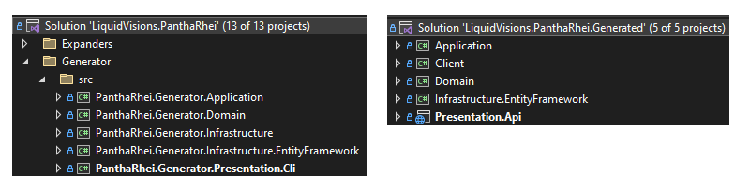
\includegraphics[width=1\textwidth]{figures/solutions.pdf}
    \caption[Separation of component libraries]{Separation of component libraries.}
    \label{fig_solutions}
\end{figure}
\subsection{Component architecture} \label{subsec_layers}

\gls{ca} organizes their components into distinct layers. This architecture promotes the
separation of concerns, maintainability, testability, and adaptability. The following
section is a short description of each layer \parencite{robert_c_martin_clean_2018}.

\subsubsection{Domain layer}
This layer contains the application's core business objects, rules, and domain logic. Entities
represent the fundamental concepts and relationships in the problem domain and are indepen-
dent of any specific technology or framework. The domain layer focuses on encapsulating the
essential complexity of the system and should be kept as pure as possible.

\subsubsection{Application layer}
This layer contains the use cases or application-specific business rules orchestrating the
interaction between entities and external systems. Use cases define the application's
behavior regarding the actions users can perform and the expected outcomes. This layer is
responsible for coordinating the flow of data between the domain layer and the
presentation or infrastructure layers while remaining agnostic to the specifics of the
user interface or external dependencies.

\subsubsection{Presentation layer}
This layer translates data and interactions between the use cases and external actors,
such as users or external systems. Interface adapters include controllers, view models,
presenters, and data mappers, which handle user input, format data for display, and
convert data between internal and external representations. The presentation layer should
be as thin as possible, focusing on the mechanics of user interaction and deferring
application logic to the use cases.

\subsubsection{Infrastructure layer}
This layer contains the technical implementations of external systems and dependencies,
such as databases, web services, file systems, or third-party libraries. The
infrastructure layer provides concrete implementations of the interfaces and abstractions
defined in the other layers, allowing the core application to remain decoupled from
specific technologies or frameworks. This layer is also responsible for configuration or
initialization code to set up the system's runtime environment.

By organizing code into these layers and adhering to the principles of \gls{ca},
developers can create software systems that are more flexible, maintainable, and testable,
with well-defined boundaries and separation of concerns
\subsection{The Design Elements} \label{subsec_design_elements}

In the context of \gls{ns} approach, the goal is to design a software system that is highly
modular, maintainable and testable. The accumulation of the Desing principles discussed
in chapter \ref{subsec_design_principles} leads to the following generalization of the
architecture. Each of the following elements has a crucial role to achieve the
design goals.

\subsubsection{Entities}
\textit{Entities} are the core business objects of the application, representing the fundamental
concepts and rules of the domain. They encapsulate the data and behavior that are
essential to the application's functionality.

\subsubsection{Interactors}
\textit{Interactors}, also known as Use cases, encapsulate the application's business
logic and represent specific actions that can be performed by the system. They are
responsible for coordinating the work of other components and ensuring that the system
behaves correctly.

\subsubsection{RequestModels}
\textit{RequestModels} are used to represent the data required by a specific interactor. They
provide a clear and concise representation of the data required by the Use Case, making it
easier to manage and modify the application.

\subsubsection{ViewModels}
ViewModels are part of the presentation layer and are responsible for managing the state
of the user interface. They receive data from the Presenters and update the user interface
accordingly. They are also responsible for handling user input and sending it to the
Controllers for processing.

\subsubsection{Controllers}
\textit{Controllers} are responsible for handling requests from the user interface and
routing them to the appropriate Interactor. They are typically part of the user interface
layer and are responsible for coordinating the work of other components.

\subsubsection{Presenters}
\textit{Presenters} are responsible for formatting and presenting data to the user
interface. They receive data from the Interactor and convert it into a format that can be
easily displayed to the user. They are also responsible for handling user input and
sending it back to the Interactor for processing.

\subsubsection{Gateways}
A \textit{Gateway} provides an abstraction layer between the application and its external
dependencies, such as databases, web services, or other systems. They allow the
system to be decoupled from its external dependencies and can be easily replaced or
adapted if needed.

\subsubsection{Boundaries}
A \textit{Boundary} refers to an interface or abstraction that separates different layers
or components of a system. The purpose of these boundaries is to promote modularity,
evolvability and testability by enforcing the separation of concerns, allowing each layer
to evolve independently.
\subsection{The Dependency rule} \label{subsec_dependency_rule}

An essential aspect is described as the dependency rule. The rule states that
\textit{source code dependencies must point only inward toward higher-level policies}
(Robert C. Martin, 2018, p. 206). This ’flow of control’ is designed following the
\gls{dip} and can be represented schematically as concentric circles containing all the
components described in section \fullref{subsec_layers}. The arrows in Figure
\ref{fig_modulair_components} clearly show that the dependencies flow from the outer
layers to the inner layers. Most outer layers are historically subjected to large-scale
refactorings due to technological changes and innovation. Separating the layers and adhering
to the dependency rule ensures that the domain logic can evolve independently from
external dependencies or certain specific technologies.

\begin{figure}[H]
    \centering
    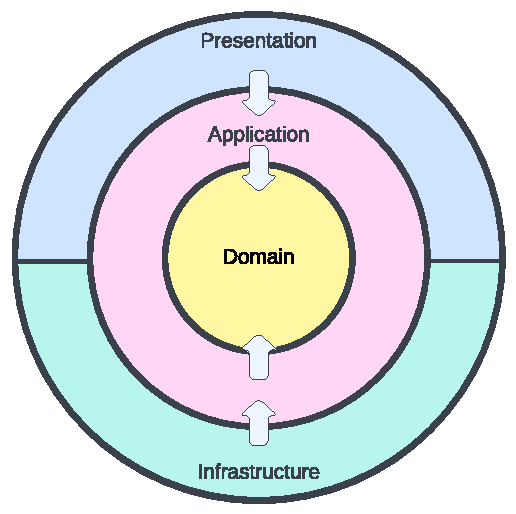
\includegraphics[width=0.4\textwidth]{figures/ca_diagram.pdf}
    \caption[Flow of control]{Flow of control}
    \label{fig_modulair_components}
\end{figure}
